\documentclass[aspectratio=169]{beamer}
\newif\iflightmode
\lightmodetrue

% ==== BEGIN COPPERFLAME COLORS ====
\usepackage{xcolor}

\definecolor{base00}{HTML}{111111}
\definecolor{base01}{HTML}{1B1B1B}
\definecolor{base02}{HTML}{303030}
\definecolor{base03}{HTML}{5E5E5E}
\definecolor{base04}{HTML}{919191}
\definecolor{base05}{HTML}{C6C6C6}
\definecolor{base06}{HTML}{E6E6E6}
\definecolor{base07}{HTML}{FFFFFF}
\definecolor{base08}{HTML}{ED4F5A}
\definecolor{base09}{HTML}{3DA794}
\definecolor{base0A}{HTML}{578158}
\definecolor{base0B}{HTML}{569CD6}
\definecolor{base0C}{HTML}{718C48}
\definecolor{base0D}{HTML}{40AB31}
\definecolor{base0E}{HTML}{755DB4}
\definecolor{base0F}{HTML}{736299}
\definecolor{baseF0}{HTML}{001100}
\definecolor{baseF1}{HTML}{001B00}
\definecolor{baseF2}{HTML}{003000}
\definecolor{baseF3}{HTML}{005E00}
\definecolor{baseF4}{HTML}{009100}
\definecolor{baseF5}{HTML}{00C600}
\definecolor{baseF6}{HTML}{00E600}
\definecolor{baseF7}{HTML}{00FF00}
\definecolor{baseF8}{HTML}{0A0014}
\definecolor{baseF9}{HTML}{140423}
\definecolor{baseFA}{HTML}{19083D}
\definecolor{baseFB}{HTML}{21096A}
\definecolor{baseFC}{HTML}{2D0A99}
\definecolor{baseFD}{HTML}{3404C9}
\definecolor{baseFE}{HTML}{3A01E8}
\definecolor{baseFF}{HTML}{4000FF}

\colorlet{foreground}{base01}
\colorlet{background}{base07}
\colorlet{foreground-secondary}{base03}
\colorlet{background-secondary}{base06}

\colorlet{shadow}{base03}

\colorlet{highlight}{baseF4}
% ===== END COPPERFLAME COLORS =====

\usepackage{fontspec}         % ttf fonts
\usepackage[skins]{tcolorbox} % floating boxes
\usepackage{tikz}             % graphics
\usepackage{calc}             % size calculations
\usepackage{beamerbaseframe}
\usepackage{beamerbasemisc}
\usepackage{beamerbasetemplates}
\usetikzlibrary{calc}         % \coordinate

% language
\usepackage[babelshorthands=true,localmarks=true]{polyglossia}
\setdefaultlanguage{de-DE}
\usepackage[
    de-DE
]{datetime2}                  % date format

% biblatex
\usepackage{csquotes}
\usepackage[style=ieee,]{biblatex}
\addbibresource{praesentationskurs.bib}

% ==== BEGIN PANDOC ====
\usepackage{hyperref} % hyperlinks, pdf metadata
\usepackage{ulem}     % striketrough
\providecommand{\tightlist}{\setlength{\itemsep}{0pt}\setlength{\parskip}{0pt}}

\usepackage{longtable,booktabs,array}
\usepackage{beamerbasetitle}
\usepackage{beamerbasesection}
\usepackage{beamerbaseoverlay}

\hypersetup{
        pdftitle={Wissenschaftliches Schreiben mit ~und },
            pdfauthor={Nico Jansen},
            pdflang={de-DE},
            pdfcreator={LaTeX via pandoc using the copperflame theme},
}

\title{Wissenschaftliches Schreiben mit \LaTeX~und \textsc{Bib}\TeX}
\author{Nico Jansen}
\date{\today}

\usepackage{color}
\usepackage{fancyvrb}
\newcommand{\VerbBar}{|}
\newcommand{\VERB}{\Verb[commandchars=\\\{\}]}
\DefineVerbatimEnvironment{Highlighting}{Verbatim}{commandchars=\\\{\}}
% Add ',fontsize=\small' for more characters per line
\usepackage{framed}
\definecolor{shadecolor}{RGB}{230,230,230}
\newenvironment{Shaded}{\begin{snugshade}}{\end{snugshade}}
\newcommand{\AlertTok}[1]{\textcolor[rgb]{0.93,0.31,0.35}{\textbf{\textit{#1}}}}
\newcommand{\AnnotationTok}[1]{\textcolor[rgb]{0.34,0.51,0.35}{#1}}
\newcommand{\AttributeTok}[1]{\textcolor[rgb]{0.44,0.55,0.28}{#1}}
\newcommand{\BaseNTok}[1]{\textcolor[rgb]{0.34,0.61,0.84}{#1}}
\newcommand{\BuiltInTok}[1]{\textcolor[rgb]{0.25,0.67,0.19}{\textbf{#1}}}
\newcommand{\CharTok}[1]{\textcolor[rgb]{0.45,0.38,0.60}{#1}}
\newcommand{\CommentTok}[1]{\textcolor[rgb]{0.57,0.57,0.57}{\textit{#1}}}
\newcommand{\CommentVarTok}[1]{\textcolor[rgb]{0.25,0.67,0.19}{\textit{#1}}}
\newcommand{\ConstantTok}[1]{\textcolor[rgb]{0.34,0.61,0.84}{#1}}
\newcommand{\ControlFlowTok}[1]{\textcolor[rgb]{0.25,0.67,0.19}{\textbf{#1}}}
\newcommand{\DataTypeTok}[1]{\textcolor[rgb]{0.24,0.65,0.58}{#1}}
\newcommand{\DecValTok}[1]{\textcolor[rgb]{0.34,0.61,0.84}{#1}}
\newcommand{\DocumentationTok}[1]{\textcolor[rgb]{0.57,0.57,0.57}{#1}}
\newcommand{\ErrorTok}[1]{\textcolor[rgb]{0.93,0.31,0.35}{#1}}
\newcommand{\ExtensionTok}[1]{\textcolor[rgb]{0.25,0.67,0.19}{#1}}
\newcommand{\FloatTok}[1]{\textcolor[rgb]{0.34,0.61,0.84}{#1}}
\newcommand{\FunctionTok}[1]{\textcolor[rgb]{0.34,0.51,0.35}{#1}}
\newcommand{\ImportTok}[1]{\textcolor[rgb]{0.25,0.67,0.19}{#1}}
\newcommand{\InformationTok}[1]{\textcolor[rgb]{0.19,0.19,0.19}{#1}}
\newcommand{\KeywordTok}[1]{\textcolor[rgb]{0.25,0.67,0.19}{\textbf{#1}}}
\newcommand{\NormalTok}[1]{\textcolor[rgb]{0.19,0.19,0.19}{#1}}
\newcommand{\OperatorTok}[1]{\textcolor[rgb]{0.19,0.19,0.19}{#1}}
\newcommand{\OtherTok}[1]{\textcolor[rgb]{0.19,0.19,0.19}{#1}}
\newcommand{\PreprocessorTok}[1]{\textcolor[rgb]{0.46,0.36,0.71}{#1}}
\newcommand{\RegionMarkerTok}[1]{\textcolor[rgb]{0.46,0.36,0.71}{#1}}
\newcommand{\SpecialCharTok}[1]{\textcolor[rgb]{0.46,0.36,0.71}{#1}}
\newcommand{\SpecialStringTok}[1]{\textcolor[rgb]{0.45,0.38,0.60}{#1}}
\newcommand{\StringTok}[1]{\textcolor[rgb]{0.45,0.38,0.60}{#1}}
\newcommand{\VariableTok}[1]{\textcolor[rgb]{0.44,0.55,0.28}{#1}}
\newcommand{\VerbatimStringTok}[1]{\textcolor[rgb]{0.19,0.19,0.19}{#1}}
\newcommand{\WarningTok}[1]{\textcolor[rgb]{0.93,0.31,0.35}{#1}}

\ifcsname Shaded\endcsname
\else
    \newenvironment{Shaded}{}{}
    \colorlet{shadecolor}{background-secondary}
\fi
\renewtcolorbox{Shaded}{
    enhanced,
    colback=shadecolor,
    colframe=shadecolor,
    opacityback=0.8,
    boxrule=0pt,
    left=0.5em, right=0.5em, top=0.5em, bottom=0.5em,
    arc=0.5em,
    auto outer arc,
interior style={fill tile image*={height=64pt}{/nix/store/67ygglrdqjjn933559bvp52w0dgr1kyv-copperflame/assets/acrylic-texture.png}},
    drop fuzzy shadow=shadow
}
% ===== END PANDOC =====

% ==== BEGIN FONTS ====
\newfontfamily{\robotoslab}{RobotoSlab}[
    Path = /nix/store/pw7l75wjxka7zyps8an64i98pddxc1z5-roboto-slab-2.000/share/fonts/truetype/,
    Extension = .ttf,
    UprightFont = *-Regular,
    BoldFont = *-Bold,
    NFSSFamily=robotoslab,
    Scale=1,
    AutoFakeSlant=0.2
]
\newfontfamily{\jbmono}{JetBrainsMono}[
    Path = /nix/store/iyn0a4mrpa3cigaashxz4l0rgcipx6cq-jetbrains-mono-2.304/share/fonts/truetype/,
    Extension = .ttf,
    UprightFont = *-Regular,
    BoldFont = *-Bold,
    ItalicFont = *-Italic,
    BoldItalicFont = *-BoldItalic,
    NFSSFamily=jbmono,
    Scale=1
]
\newfontfamily{\dosfont}{less-perfect-dos-vga}[
    Path = /nix/store/2q3f42n9lbfaqass2qdsxymph7bsral6-perfect-dos-vga/share/fonts/truetype/,
    Extension = .ttf,
    NFSSFamily=dosfont,
    Scale=1.2
]

\renewcommand{\rmdefault}{robotoslab}
\renewcommand{\sfdefault}{robotoslab}
\renewcommand{\ttdefault}{jbmono}
\renewcommand{\familydefault}{\sfdefault}

% https://tex.stackexchange.com/questions/460233/redefine-em-to-use-slshape
\makeatletter
\DeclareRobustCommand\em{\@nomath\em \ifdim \fontdimen\@ne\font >\z@ \eminnershape \else \slshape \fi}
\DeclareTextFontCommand{\emph}{\em}
\makeatother
% ===== END FONTS =====

% ==== BEGIN BEAMER FONTS ====
\setbeamerfont{frametitle}{family=\robotoslab}
\setbeamerfont{title}{family=\robotoslab}
\setbeamerfont{subtitle}{family=\robotoslab}
\setbeamerfont{author}{family=\robotoslab}
\setbeamerfont{date}{parent=author}
\setbeamerfont{institute}{family=\robotoslab}
\setbeamerfont{section title}{parent=title}
\setbeamerfont{subsection title}{parent=subtitle}
% ==== BEGIN BEAMER FONTS ====

% ==== BEGIN COMMON ====

\newcommand\citestyle[1]{\textcolor{foreground-secondary}{\textsuperscript{#1}}}
\newcommand\citationneeded{\citestyle{[citation needed]}}
\let\oldcite=\cite
\renewcommand{\cite}[1]{\citestyle{\oldcite{#1}}}
\let\oldautocite\autocite
\renewcommand{\autocite}[1]{\citestyle{\oldautocite{#1}}}
% ===== END COMMON =====

% ==== BEGIN BEAMER COLORS ====
\setbeamercolor{background canvas}{bg=background}
\setbeamercolor{normal text}{fg=foreground}
\setbeamercolor{alerted text}{fg=highlight}
\setbeamercolor{structure}{fg=foreground}
\setbeamercolor{subsection title}{fg=foreground}

\setbeamercolor{bibliography item}{parent=item,fg=highlight}
\setbeamercolor{bibliography entry author}{use=structure,fg=normal text.fg}
\setbeamercolor{bibliography entry title}{use=normal text,fg=normal text.fg}
\setbeamercolor{bibliography entry location}{use=structure,fg=foreground-secondary}
\setbeamercolor{bibliography entry note}{use=structure,fg=foreground-secondary}
% ===== END BEAMER COLORS =====

% ==== BEGIN BEAMER TEMPLATE ====

\newcommand\titleline{
    \usebeamerfont{title}
    \begin{tikzpicture}
        \node[anchor=center, inner xsep=0pt] {
            \begin{tikzpicture}
                \fill[highlight] (0,0) rectangle (\textwidth, 1pt);
            \end{tikzpicture}
        };
    \end{tikzpicture}
}

\setbeamertemplate{title page}{
    \vfill
    {\usebeamercolor[fg]{title}\usebeamerfont{title}\inserttitle}
    \\
    {\usebeamercolor[fg]{subtitle}\usebeamerfont{subtitle}\insertsubtitle}
    \titleline
    \\
    {\usebeamercolor[fg]{author}\usebeamerfont{author}\insertauthor}
    \hfill
    {\usebeamercolor[fg]{date}\usebeamerfont{date}\insertdate}
    \\
    {\usebeamercolor[fg]{institute}\usebeamerfont{institute}\insertinstitute}
    \vfill
}

\newcommand\currentsection{}
\newcommand\currentsubsection{}

\AtBeginSection[]{
    \renewcommand\currentsection{\insertsection}
    \renewcommand\currentsubsection{}
}

\AtBeginSubsection[]{
    \renewcommand\currentsubsection{\insertsubsection}
}

% Does not seem to work properly
\newcommand{\mksectiontitle}{
    \vfill
    {\usebeamercolor[fg]{section title}\usebeamerfont{section title}\currentsection}
    \leavevmode\\
    \titleline
    \\
    {\usebeamercolor[fg]{subsection title}\usebeamerfont{subsection title}\currentsubsection}
    \vfill
}

\newtcolorbox{FrameTitle}{
    enhanced,
    colback=shadecolor,
    colframe=shadecolor,
    opacityback=0.8,
    boxrule=0pt,
    sharp corners,
    nobeforeafter,
    top = 4pt, bottom = 4pt,
    interior style={fill tile image*={height=64pt}{/nix/store/67ygglrdqjjn933559bvp52w0dgr1kyv-copperflame/assets/acrylic-texture.png}},
    fuzzy shadow={0mm}{-2pt}{0mm}{0.5pt}{shadow}
}
\setbeamertemplate{frametitle}{%
    \nointerlineskip%
    \begin{beamercolorbox}[wd=\paperwidth]{frametitle}%
        \begin{FrameTitle}%
            \begin{beamercolorbox}[sep=0pt]{frametitle}%
                \usebeamerfont{frametitle}%
                \strut\insertframetitle\strut%
            \end{beamercolorbox}%
        \end{FrameTitle}%
    \end{beamercolorbox}%
}

\setbeamertemplate{frametitle continuation}{\insertcontinuationcount}

\newlength{\progressHeight}%
\newlength{\progressLength}%
\setbeamertemplate{footline}{%
        \begin{beamercolorbox}[wd=\textwidth, sep=3ex]{footline}%
        \hfill%
        \insertframenumber\color{foreground-secondary}{/\inserttotalframenumber}%
    \end{beamercolorbox}%
        
    \setlength{\progressHeight}{1pt}%
    \setlength{\progressLength}{\paperwidth * \ratio{\insertframenumber pt}{\inserttotalframenumber pt}}%
    \begin{tikzpicture}%
        \fill[background-secondary] (0,0) rectangle (\paperwidth, \progressHeight);%
        \fill[highlight] (0,0) rectangle (\progressLength, \progressHeight);%
    \end{tikzpicture}%
    
}

\setbeamertemplate{navigation symbols}{}
\setbeamertemplate{itemize items}[circle]
\setbeamertemplate{bibliography item}{\insertbiblabel}

% ===== END BEAMER TEMPLATE =====

% ==== BEGIN HEADER INCLUDES ====
\usepackage[babelshorthands=true,localmarks=true]{polyglossia}
\setdefaultlanguage{de-DE}

\usepackage[color=highlight]{attachfile2}

\usepackage{hologo}

\hypertarget{various-tex-logos}{%
\section{various TeX logos}\label{various-tex-logos}}

\newcommand\BibTeX{\textsc{Bib}\TeX}
\newcommand\BibLaTeX{\textsc{Bib}\LaTeX}

\newcommand{\lmr}{\fontfamily{lmr}\selectfont}
\newcommand{\lmss}{\fontfamily{lmss}\selectfont}
\newcommand{\lmtt}{\fontfamily{lmtt}\selectfont}

\renewcommand\mathfamilydefault{lmr}

\newtcolorbox{OutputBox}{
    enhanced jigsaw,
    % colback=background,
    % colframe=background,
    opacityback=0,
    % boxrule=0pt,
    frame hidden,
    left=0.5em, right=0.5em, top=0.5em, bottom=0.5em,
}
\newenvironment{Output}{
    \begin{OutputBox}
    \begin{beamercolorbox}{foreground text}
        \lmr % Render simulated output in Latin Modern
}{
        \end{beamercolorbox}
    \end{OutputBox}
}

\newcommand{\link}[1]{\alert{\underline{#1}}}

\newenvironment{cmddef}[1]{
    \alert{\ttfamily #1}
    \begin{quote}\upshape
}{
    \end{quote}
}

% ===== END HEADER INCLUDES =====

\begin{document}

        \begin{frame}
            \maketitle
            \iflightmode
            \else
                \textcolor{foreground-secondary}{
                    Hinweis: Es ist auch eine 
                    \textattachfile[mimetype=application/x-pdf]{praesentationskurs-light.pdf}{\alert{\underline{helle Version}}}
                    an diese PDF angehängt. \\
                    (kein Weblink, funktioniert nicht in jedem PDF-Reader! Getestet mit \href{https://okular.kde.org)}{\alert{\underline{Okular}}}.)
                }
            \fi
        \end{frame}

    
        
    \begin{frame}[fragile]{Ein \LaTeX-Dokument}
    \protect\hypertarget{ein--dokument}{}
    \begin{minipage}{0.66\textwidth}

\begin{Shaded}
\begin{Highlighting}[]
\BuiltInTok{\textbackslash{}documentclass}\NormalTok{[a4paper]\{}\ExtensionTok{article}\NormalTok{\}}
\KeywordTok{\textbackslash{}begin}\NormalTok{\{}\ExtensionTok{document}\NormalTok{\}}
    \FunctionTok{\textbackslash{}textbf}\NormalTok{\{Hallo Welt!\}}
\KeywordTok{\textbackslash{}end}\NormalTok{\{}\ExtensionTok{document}\NormalTok{\}}
\end{Highlighting}
\end{Shaded}

    \end{minipage}\begin{minipage}{0.33\textwidth}

    \bgroup 
        \begin{OutputBox}
        \begin{beamercolorbox}{foreground text}
            \fontfamily{lmr}\selectfont% Render simulated output in Latin Modern

        \textbf{Hallo Welt!}

            \end{beamercolorbox}
        \end{OutputBox}
    \egroup

    \end{minipage}

    \vspace{0.5\baselineskip}

    \textbf{Kompilieren:}

\begin{Shaded}
\begin{Highlighting}[]
\NormalTok{$ latex beispiel.tex}
\end{Highlighting}
\end{Shaded}

    Erzeugt \texttt{beispiel.dvi}.\\
    \strut \\
    \emph{pdflatex}\autocite{ctan-pdftex},
    \emph{xelatex}\autocite{ctan-xetex} und
    \emph{lualatex}\autocite{ctan-luatex} geben PDF aus.\\
    (\hologo{XeTeX} und \hologo{LuaTeX} unterstützen auch Unicode und
    TrueType Schriftarten).
    \end{frame}

    \begin{frame}{Fakten über \LaTeX}
    \protect\hypertarget{fakten-uxfcber}{}
    \begin{itemize}
    \tightlist
    \item
      \enquote{[\ldots] a system for typesetting documents}\autocite{latex}
    \item
      Erlaubt es Dokumente aus Code zu erzeugen\autocite{latex}

      \begin{itemize}
      \tightlist
      \item
        Inhalt größtenteils unabhängig vom Design (im Gegensatz zu einem
        \emph{WYSIWYG}-Editor)\autocite{latex}
      \item
        Umfassende Syntax für mathematische Ausdrücke\autocite{latex}
      \item
        Verschiedene Ausgabeformate (DVI\autocite{latex},
        PostScript\autocite{ctan-dvips}, PDF\autocite{ctan-dvipdfmx},
        \ldots)
      \end{itemize}
    \item
      Erschienen 1985 in Version 2.09. Aktuell ist
      \hologo{LaTeX2e}\autocite{latex}
    \item
      Standard in der Wissenschaft \autocite{latex}
    \item
      Erweiterbar mit über 6000 Paketen von
      \href{https://ctan.org}{\alert{\underline{CTAN}}}\autocite{ctan}
    \end{itemize}
    \end{frame}

    \begin{frame}[fragile]{\LaTeX-Befehle}
    \protect\hypertarget{befehle}{}
    \bgroup 
        \alert{\ttfamily \textbackslash name\{args\} \\ \textbackslash name[optional]\{args\}}
        \begin{quote}\upshape

        Führt \textbackslash name mit den Argumenten \enquote{\ttfamily args} und \enquote{\ttfamily optional} aus.\cite{latex}

        \end{quote}
    \egroup

    \bgroup 
        \alert{\ttfamily \textbackslash newcommand\{\textbackslash name\}[$n$]\{Definition\}}
        \begin{quote}\upshape

        Definiert einen neuen Befehl \textbackslash name mit $n$ (oder 0) Argumenten als \enquote{\ttfamily Definition}.
        Die Argumente können mit \texttt{\#1}, \texttt{\#2}, \ldots\ verwendet werden.\cite{latex}

        \end{quote}
    \egroup

    \bgroup 
        \alert{\ttfamily \textbackslash begin\{env\} \\ \textbackslash end\{env\}}
        \begin{quote}\upshape

        Beginnt und beendet eine Umgebung namens \enquote{\ttfamily env}.\cite{latex}

        \end{quote}
    \egroup

    \bgroup 
        \alert{\ttfamily \textbackslash newenvironment\{env\}[$n$]\{vorher\}\{nachher\}}
        \begin{quote}\upshape

        Definiert eine neue Umgebung namens \enquote{\ttfamily env} mit \enquote{\ttfamily vorher} und \enquote{\ttfamily nachher} vor und nach dem Inhalt und $n$ (oder 0) Argumenten.\cite{latex}

        \end{quote}
    \egroup

    \emph{Zum Überschreiben}: \texttt{\textbackslash{}renewcommand} und
    \texttt{\textbackslash{}renewenvironment}\autocite{latex}
    \end{frame}

    \begin{frame}[fragile]{Einige häufig verwendete Befehle 1}
    \protect\hypertarget{einige-huxe4ufig-verwendete-befehle-1}{}
    \begin{minipage}{0.66\textwidth}

\begin{Shaded}
\begin{Highlighting}[]
\FunctionTok{\textbackslash{}textbf}\NormalTok{\{fett\}, \{}\FunctionTok{\textbackslash{}bfseries}\NormalTok{ fett\} }\FunctionTok{\textbackslash{}\textbackslash{}}
\FunctionTok{\textbackslash{}textit}\NormalTok{\{kursiv\}, \{}\FunctionTok{\textbackslash{}itshape}\NormalTok{ kursiv\} }\FunctionTok{\textbackslash{}\textbackslash{}}
\FunctionTok{\textbackslash{}textsl}\NormalTok{\{geneigt\}, \{}\FunctionTok{\textbackslash{}slshape}\NormalTok{ geneigt\}}\FunctionTok{\textbackslash{}\textbackslash{}}
\FunctionTok{\textbackslash{}texttt}\NormalTok{\{mono\}, \{}\FunctionTok{\textbackslash{}ttfamily}\NormalTok{ mono\} }\FunctionTok{\textbackslash{}\textbackslash{}}
\FunctionTok{\textbackslash{}emph}\NormalTok{\{sehr }\FunctionTok{\textbackslash{}emph}\NormalTok{\{sehr\} wichtig\} }\FunctionTok{\textbackslash{}\textbackslash{}}
\NormalTok{Fußnoten}\FunctionTok{\textbackslash{}footnote}\NormalTok{\{Hier unten!\} }\FunctionTok{\textbackslash{}\textbackslash{}}
\FunctionTok{\textbackslash{}small}\NormalTok{ klein }\FunctionTok{\textbackslash{}large}\NormalTok{ groß}
\FunctionTok{\textbackslash{}Large}\NormalTok{ größer }\FunctionTok{\textbackslash{}normalsize}
\CommentTok{\% Ein Kommentar}
\end{Highlighting}
\end{Shaded}

    \end{minipage}\begin{minipage}{0.33\textwidth}

    \bgroup 
        \begin{OutputBox}
        \begin{beamercolorbox}{foreground text}
            \fontfamily{lmr}\selectfont% Render simulated output in Latin Modern

    \textbf{fett}, {\bfseries fett} \\
    \textit{kursiv}, {\itshape kursiv} \\
    \textsl{geneigt}, {\slshape geneigt}\\
    {\fontfamily{lmtt}\selectfont mono}, {\fontfamily{lmtt}\selectfont mono} \\
    \emph{sehr \emph{sehr} wichtig} \\
    Fußnoten\footnote{\fontfamily{lmr}\selectfont Hier unten!} \\
    \small klein \large groß
    \Large größer \normalsize
    % Ein Kommentar

            \end{beamercolorbox}
        \end{OutputBox}
    \egroup

    \end{minipage}
    \end{frame}

    \begin{frame}[fragile]{Einige häufig verwendete Befehle 2}
    \protect\hypertarget{einige-huxe4ufig-verwendete-befehle-2}{}
    \begin{minipage}{0.66\textwidth}

\begin{Shaded}
\begin{Highlighting}[]
\KeywordTok{\textbackslash{}begin}\NormalTok{\{}\ExtensionTok{itemize}\NormalTok{\}}
    \FunctionTok{\textbackslash{}item}\NormalTok{ Einige}
    \FunctionTok{\textbackslash{}item}\NormalTok{ Stichpunkte}
    \KeywordTok{\textbackslash{}begin}\NormalTok{\{}\ExtensionTok{enumerate}\NormalTok{\}}
        \FunctionTok{\textbackslash{}item}\NormalTok{ Eine}
        \FunctionTok{\textbackslash{}item}\NormalTok{ Aufzählung}
    \KeywordTok{\textbackslash{}end}\NormalTok{\{}\ExtensionTok{enumerate}\NormalTok{\}}
\KeywordTok{\textbackslash{}end}\NormalTok{\{}\ExtensionTok{itemize}\NormalTok{\}}

\KeywordTok{\textbackslash{}begin}\NormalTok{\{}\ExtensionTok{description}\NormalTok{\}}
    \FunctionTok{\textbackslash{}item}\NormalTok{[}\FunctionTok{\textbackslash{}TeX}\NormalTok{] Ein Textsatzsystem }
    \FunctionTok{\textbackslash{}item}\NormalTok{[Löwe] }\FunctionTok{\textbackslash{}TeX}\NormalTok{ Maskottchen }
\KeywordTok{\textbackslash{}end}\NormalTok{\{}\ExtensionTok{description}\NormalTok{\}}
\end{Highlighting}
\end{Shaded}

    \end{minipage}\begin{minipage}{0.33\textwidth}

    \bgroup 
        \begin{OutputBox}
        \begin{beamercolorbox}{foreground text}
            \fontfamily{lmr}\selectfont% Render simulated output in Latin Modern

    \begin{itemize}
        \item Einige
        \item Stichpunkte
        \begin{enumerate}
            \item Eine
            \item Aufzählung
        \end{enumerate}
    \end{itemize}

    \begin{description}
        \item[\TeX] Ein Textsatzsystem
        \item[Löwe] Das \TeX\ Maskottchen
    \end{description}

            \end{beamercolorbox}
        \end{OutputBox}
    \egroup

    \end{minipage}
    \end{frame}

    \begin{frame}[fragile]{Mathematische Formeln}
    \protect\hypertarget{mathematische-formeln}{}
    \begin{minipage}{0.66\textwidth}

\begin{Shaded}
\begin{Highlighting}[]
\NormalTok{Daher ist }\SpecialStringTok{\textbackslash{}(x=4\textbackslash{})}\NormalTok{. }\CommentTok{\% oder $...$}
\SpecialStringTok{\textbackslash{}[}
\SpecialStringTok{  x\_\{1,2\} = {-}}\SpecialCharTok{\textbackslash{}frac}\SpecialStringTok{\{p\}\{2\}}\SpecialCharTok{\textbackslash{}pm}
\SpecialStringTok{  }\SpecialCharTok{\textbackslash{}sqrt}\SpecialStringTok{\{}\SpecialCharTok{\textbackslash{}left}\SpecialStringTok{(}\SpecialCharTok{\textbackslash{}frac}\SpecialStringTok{\{p\}\{2\}}\SpecialCharTok{\textbackslash{}right}\SpecialStringTok{)\^{}2{-}q\}}
\SpecialStringTok{\textbackslash{}]} \CommentTok{\% oder $$...$$}
\KeywordTok{\textbackslash{}begin}\NormalTok{\{}\ExtensionTok{align*}\NormalTok{\}}
\SpecialStringTok{  0   =\& 5x + 25 \&\& {-}25 }\SpecialCharTok{\textbackslash{}\textbackslash{}}
\SpecialStringTok{  {-}25 =\& 5x      \&\& /{-}5 }\SpecialCharTok{\textbackslash{}\textbackslash{}}
\SpecialStringTok{  5   =\& x}
\KeywordTok{\textbackslash{}end}\NormalTok{\{}\ExtensionTok{align*}\NormalTok{\}}
\SpecialStringTok{$$ }\SpecialCharTok{\textbackslash{}sum\textbackslash{}limits}\SpecialStringTok{\_\{i=1\}\^{}n i }
\SpecialStringTok{   }\SpecialCharTok{\textbackslash{}leq}\SpecialStringTok{ }\SpecialCharTok{\textbackslash{}prod\textbackslash{}limits}\SpecialStringTok{\_\{i=1\}\^{}n i $$}
\SpecialStringTok{$ }\SpecialCharTok{\textbackslash{}in}\SpecialStringTok{, }\SpecialCharTok{\textbackslash{}cup}\SpecialStringTok{, }\SpecialCharTok{\textbackslash{}cap}\SpecialStringTok{, }\SpecialCharTok{\textbackslash{}land}\SpecialStringTok{, }\SpecialCharTok{\textbackslash{}lor}\SpecialStringTok{, }\SpecialCharTok{\textbackslash{}pi}\SpecialStringTok{ $}
\end{Highlighting}
\end{Shaded}

    \end{minipage}\begin{minipage}{0.33\textwidth}

    \bgroup 
        \begin{OutputBox}
        \begin{beamercolorbox}{foreground text}
            \fontfamily{lmr}\selectfont% Render simulated output in Latin Modern

    Daher ist \(x=4\). % oder $...$
    \[
        x_{1,2} = -\frac{p}{2}\pm
        \sqrt{\left(\frac{p}{2}\right)^2-q}
    \] % oder $$...$$
    \begin{align*}
      0   =& 5x + 25 && -25 \\
      -25 =& 5x      && /-5 \\
      5   =& x
    \end{align*}
    $$ \sum\limits_{i=1}^n i 
       \leq \prod\limits_{i=1}^n i $$
    $ \in, \cup, \cap, \land, \lor, \pi $

            \end{beamercolorbox}
        \end{OutputBox}
    \egroup

    \end{minipage}

    Beim finden anderer Symbole hilft
    \href{https://detexify.kirelabs.org/classify.html}{\alert{\underline{Detexify}}}.\autocite{detexify}
    \end{frame}

    \begin{frame}[fragile]{Zitate 1}
    \protect\hypertarget{zitate-1}{}
    \begin{minipage}{0.66\textwidth}

\begin{Shaded}
\begin{Highlighting}[]
\BuiltInTok{\textbackslash{}documentclass}\NormalTok{\{}\ExtensionTok{article}\NormalTok{\}}
\KeywordTok{\textbackslash{}begin}\NormalTok{\{}\ExtensionTok{document}\NormalTok{\}}
\NormalTok{\textasciigrave{}\textasciigrave{}Today ... paper\textquotesingle{}\textquotesingle{} }\KeywordTok{\textbackslash{}cite}\NormalTok{\{}\ExtensionTok{latex}\NormalTok{\}}

\KeywordTok{\textbackslash{}begin}\NormalTok{\{}\ExtensionTok{thebibliography}\NormalTok{\}\{9\}}
    \FunctionTok{\textbackslash{}bibitem}\NormalTok{\{latex\} }
\NormalTok{    L. Lamport, }\FunctionTok{\textbackslash{}LaTeX}\NormalTok{, 1994.}
\KeywordTok{\textbackslash{}end}\NormalTok{\{}\ExtensionTok{thebibliography}\NormalTok{\}}
\KeywordTok{\textbackslash{}end}\NormalTok{\{}\ExtensionTok{document}\NormalTok{\}}
\end{Highlighting}
\end{Shaded}

    \end{minipage}\begin{minipage}{0.33\textwidth}

    \bgroup 
        \begin{OutputBox}
        \begin{beamercolorbox}{foreground text}
            \fontfamily{lmr}\selectfont% Render simulated output in Latin Modern

    ``Today you are likely to send a 
    document electronically -- by e-mail 
    or on a diskette -- 
    rather than on paper'' [\textbf{?}]
    \\ \\
    \textbf{\Large References}

    [1] L. Lamport, \LaTeX, 1994.

            \end{beamercolorbox}
        \end{OutputBox}
    \egroup

    \end{minipage}

    \begin{itemize}
    \tightlist
    \item
      Quellen in \texttt{\textbackslash{}thebibliography} angegeben
      \autocite{overleaf-bibtex}
    \item
      \texttt{\textbackslash{}cite\{key\}} fügt Referenz zu
      \enquote{key} ein \autocite{overleaf-bibtex}
    \item
      Referenzen werden noch nicht richtig aufgelöst, sondern als
      \mbox{\fontfamily{lmr}\selectfont[\textbf{?}]} angezeigt
    \end{itemize}

    \textcolor{foreground-secondary}{\tiny Der Eintrag wurde aus Platzgründen gekürzt. Der vollständige Eintrag ist unter \cite{latex} im Quellenverzeichnis zu finden.}
    \end{frame}

    \begin{frame}[fragile]{Zitate 2}
    \protect\hypertarget{zitate-2}{}
    \begin{minipage}{0.66\textwidth}

\begin{Shaded}
\begin{Highlighting}[]
\NormalTok{$ xelatex zitate.tex}
\NormalTok{...}
\NormalTok{LaTeX Warning: There were }
\NormalTok{    undefined references.}
\NormalTok{LaTeX Warning: Label(s) may have }
\NormalTok{    changed. Rerun to get }
\NormalTok{    cross{-}references right}
\NormalTok{...}
\NormalTok{$ xelatex zitate.tex}
\NormalTok{...    }
\end{Highlighting}
\end{Shaded}

    \end{minipage}\begin{minipage}{0.33\textwidth}

    \bgroup 
        \begin{OutputBox}
        \begin{beamercolorbox}{foreground text}
            \fontfamily{lmr}\selectfont% Render simulated output in Latin Modern

    ``Today you are likely to send a 
    document electronically -- by e-mail 
    or on a diskette -- 
    rather than on paper'' [1]
    \\ \\
    \textbf{\Large References}

    [1] L. Lamport, \LaTeX, 1994.

            \end{beamercolorbox}
        \end{OutputBox}
    \egroup

    \end{minipage}

    \begin{itemize}
    \tightlist
    \item
      \LaTeX~muss zweimal ausgeführt werden \autocite{overleaf-bibtex}

      \begin{enumerate}
      \tightlist
      \item
        Verweise werden in \enquote{zitate.aux} geschrieben
      \item
        Verweise werden aus \enquote{zitate.aux} gelesen und korrekt
        aufgelöst
      \end{enumerate}
    \end{itemize}
    \end{frame}

    \begin{frame}[fragile]{\textsc{Bib}\TeX}
    \protect\hypertarget{section}{}
    Ersetzt \texttt{thebibliography} mit einer \texttt{.bib} Datei
    \autocite{overleaf-bibtex}\\

    \begin{minipage}{0.495\textwidth}

\begin{Shaded}
\begin{Highlighting}[]
\BuiltInTok{\textbackslash{}documentclass}\NormalTok{\{}\ExtensionTok{article}\NormalTok{\}}
\KeywordTok{\textbackslash{}begin}\NormalTok{\{}\ExtensionTok{document}\NormalTok{\}}
\NormalTok{\textasciigrave{}\textasciigrave{}Today ... paper\textquotesingle{}\textquotesingle{} }
\KeywordTok{\textbackslash{}cite}\NormalTok{\{}\ExtensionTok{latex}\NormalTok{\}}

\BuiltInTok{\textbackslash{}bibliography}\NormalTok{\{}\ExtensionTok{zitate.bib}\NormalTok{\}}
\BuiltInTok{\textbackslash{}bibliographystyle}\NormalTok{\{}\ExtensionTok{plain}\NormalTok{\}}
\KeywordTok{\textbackslash{}end}\NormalTok{\{}\ExtensionTok{document}\NormalTok{\}}
\end{Highlighting}
\end{Shaded}

    \end{minipage}\begin{minipage}{0.01\textwidth}

    \phantom{x}

    \end{minipage}\begin{minipage}{0.495\textwidth}

\begin{Shaded}
\begin{Highlighting}[]
\VariableTok{@Book}\NormalTok{\{}\OtherTok{latex}\NormalTok{,}
  \DataTypeTok{author}\NormalTok{ = \{Leslie Lamport\},}
  \DataTypeTok{publisher}\NormalTok{ = \{Pearson }
\NormalTok{      / Prentice Hall\},}
  \DataTypeTok{title}\NormalTok{ = \{}\CharTok{\textbackslash{}LaTeX}\NormalTok{ ...\},}
  \DataTypeTok{year}\NormalTok{ = \{1994\},}
\NormalTok{\}}
\end{Highlighting}
\end{Shaded}

    \centering{\textcolor{foreground-secondary}{\scriptsize zitate.bib}}

    \end{minipage}

    \vspace{0.2\baselineskip}

    \begin{minipage}{0.495\textwidth}

\begin{Shaded}
\begin{Highlighting}[]
\NormalTok{$ xelatex zitate.tex}
\NormalTok{$ bibtex zitate}
\NormalTok{$ xelatex zitate.tex}
\NormalTok{$ xelatex zitate.tex}
\end{Highlighting}
\end{Shaded}

    \end{minipage}\begin{minipage}{0.01\textwidth}

    \phantom{x}

    \end{minipage}\begin{minipage}{0.495\textwidth}

    \begin{flushleft}
    In einem Schritt mit Build-Tools wie \mbox{\emph{latexmk}}\cite{ctan-latexmk} oder \mbox{\emph{tectonic}}\cite{tectonic}
    \end{flushleft}

    \end{minipage}
    \end{frame}

    \begin{frame}[fragile]{\textsc{Bib}\TeX~- Einträge und Felder}
    \protect\hypertarget{eintruxe4ge-und-felder}{}
    \begin{minipage}{0.7\textwidth}

    \begin{longtable}[]{@{}ll@{}}
    \toprule()
    Eintragstyp & Beschreibung \\
    \midrule()
    \endhead
    \texttt{@Article} & Artikel (in einer Zeitschrift) \cite{bibtex} \\
    \texttt{@Book} & Ein Buch mit Verlag \cite{bibtex} \\
    \texttt{@Booklet} & Ein Buch ohne Verlag \cite{bibtex} \\
    \texttt{@InBook} & Teil eines Buches \cite{bibtex} \\
    \texttt{@InCollection} & Teil eines Sammelbandes \cite{bibtex} \\
    \texttt{@Manual} & Dokumentationen, Anleitungen \cite{bibtex} \\
    \texttt{@MastersThesis} & Masterarbeit \cite{bibtex} \\
    \texttt{@PhdThesis} & Doktorarbeit \cite{bibtex} \\
    \texttt{@Techreport} & Technischer Bericht \cite{bibtex} \\
    \texttt{@Unpublished} & Unveröffentlichtes Werk \cite{bibtex} \\
    \texttt{@Misc} & Alles andere \cite{bibtex} \\
    \bottomrule()
    \end{longtable}

    \end{minipage}\begin{minipage}{0.3\textwidth}

    \phantom{m}Einige Felder: \autocite{bibtex}

    \begin{itemize}
    \tightlist
    \item
      author
    \item
      title
    \item
      year
    \item
      month
    \item
      publisher
    \item
      journal
    \item
      institution
    \item
      booktitle
    \item
      volume
    \item
      chapter
    \item
      edition
    \item
      note
    \end{itemize}

    \vfill

    \end{minipage}

    Je nach Eintragstyp werden verschiedene Felder unterstützt
    \autocite{bibtex}
    \end{frame}

    \begin{frame}{Quellen für \textsc{Bib}\TeX~Einträge}
    \protect\hypertarget{quellen-fuxfcr-eintruxe4ge}{}
    \begin{minipage}{0.7\textwidth}

    Einträge können aus Suchmaschinen kopiert werden:\\

    \begin{itemize}
    \tightlist
    \item
      Google Scholar \autocite{google-scholar}
    \item
      IEEE Xplore \autocite{ieee-xplore}
    \item
      DBLP\normalsize~\autocite{dblp}

      \begin{itemize}
      \tightlist
      \item
        Auf Informatik spezialisierte Literaturdatenbank
      \item
        Über 6.000.000 Einträge
      \item
        Alle Einträge werden manuell geprüft

        \begin{itemize}
        \tightlist
        \item
          Hohe Qualität gegenüber anderen Angeboten
        \end{itemize}
      \end{itemize}
    \end{itemize}

    \end{minipage}\begin{minipage}{0.3\textwidth}

    \vfill

    \centering{\scriptsize Google Scholar}
    \hfill 
\includegraphics[width=.8\textwidth]{google-scholar.png}

    \vspace{.5\baselineskip}

    \centering{\scriptsize IEEE Xplore}
    \hfill 
\includegraphics[width=.8\textwidth]{ieee.png}

    \vspace{.5\baselineskip}

    \centering{\scriptsize DBLP}
    
\includegraphics[width=\textwidth]{dblp.png}

    \end{minipage}
    \end{frame}

    \begin{frame}[fragile]{JabRef}
    \protect\hypertarget{jabref}{}
    \begin{minipage}{0.4\textwidth}

    \begin{itemize}
    \tightlist
    \item
      GUI Editor für \texttt{.bib}-Dateien \autocite{jabref}
    \item
      Bietet eine Suchfunktion für einige wissenschaftliche Datenbanken

      \begin{itemize}
      \tightlist
      \item
        Unter anderem DBLP
      \item
        Gefundene Einträge können direkt importiert werden
      \end{itemize}
    \end{itemize}

    \end{minipage}\begin{minipage}{0.6\textwidth}

    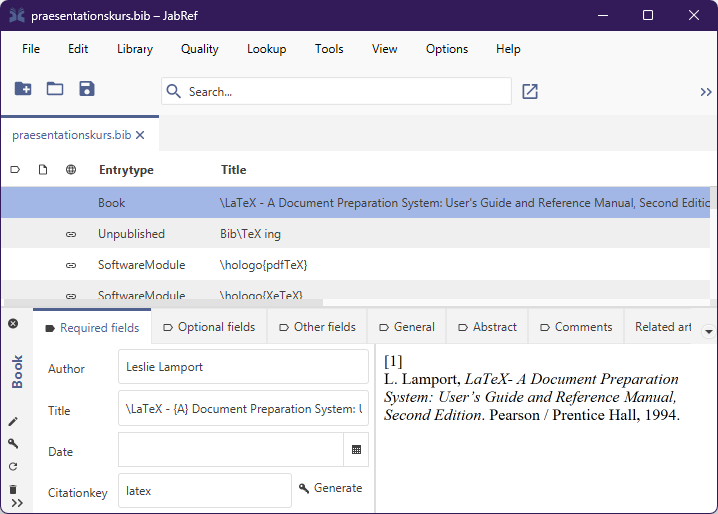
\includegraphics[width=\textwidth]{jabref.png}

    \end{minipage}
    \end{frame}

    \begin{frame}[fragile]{\textsc{Bib}\LaTeX}
    \protect\hypertarget{section-1}{}
    \begin{itemize}
    \tightlist
    \item
      Neuentwicklung des Zitiersystems von
      \LaTeX \autocite{ctan-biblatex}
    \item
      Bessere Unterstützung für Sprachen neben Englisch
      \autocite{ctan-biblatex}
    \item
      Zusätzliche Eintragstypen wie \texttt{@online}, \texttt{@software}
      und \texttt{@dataset} \autocite{biblatex}
    \item
      Kompatibel mit \textsc{Bib}\TeX~Einträgen \autocite{biblatex}
    \end{itemize}

    \begin{minipage}{0.66\textwidth}

\begin{Shaded}
\begin{Highlighting}[]
\BuiltInTok{\textbackslash{}documentclass}\NormalTok{\{}\ExtensionTok{article}\NormalTok{\}}
\BuiltInTok{\textbackslash{}usepackage}\NormalTok{[style=ieee]\{}\ExtensionTok{biblatex}\NormalTok{\}}
\FunctionTok{\textbackslash{}addbibresource}\NormalTok{\{zitate.bib\}}
\KeywordTok{\textbackslash{}begin}\NormalTok{\{}\ExtensionTok{document}\NormalTok{\}}
\NormalTok{\textasciigrave{}\textasciigrave{}Today ... paper\textquotesingle{}\textquotesingle{} }
\KeywordTok{\textbackslash{}cite}\NormalTok{\{}\ExtensionTok{latex}\NormalTok{\}}

\FunctionTok{\textbackslash{}printbibliography}
\KeywordTok{\textbackslash{}end}\NormalTok{\{}\ExtensionTok{document}\NormalTok{\}}
\end{Highlighting}
\end{Shaded}

    \end{minipage}\begin{minipage}{0.33\textwidth}

    \begin{itemize}
    \tightlist
    \item
      Muss als Paket geladen werden \autocite{biblatex}

      \begin{itemize}
      \tightlist
      \item
        Stil wird als Argument übergeben
      \end{itemize}
    \item
      \texttt{bibtex} wird durch \texttt{biber} ersetzt
      \autocite{biblatex}
    \end{itemize}

    \end{minipage}
    \end{frame}

        \begin{frame}[allowframebreaks]
            \frametitle{Quellen}
            \printbibliography[heading=none]
    \end{frame}
    
    
\end{document}